%%%%%%%%%%%%%%%%%%%%%%%%%%%%%%%%%%%%%%%%%
% Beamer Presentation
% LaTeX Template
% Version 2.0 (March 8, 2022)
%
% This template originates from:
% https://www.LaTeXTemplates.com
%
% Author:
% Vel (vel@latextemplates.com)
%
% License:
% CC BY-NC-SA 4.0 (https://creativecommons.org/licenses/by-nc-sa/4.0/)
%
%%%%%%%%%%%%%%%%%%%%%%%%%%%%%%%%%%%%%%%%%

%----------------------------------------------------------------------------------------
%	PACKAGES AND OTHER DOCUMENT CONFIGURATIONS
%----------------------------------------------------------------------------------------

\documentclass[
	9pt, % Set the default font size, options include: 8pt, 9pt, 10pt, 11pt, 12pt, 14pt, 17pt, 20pt
	t, % Uncomment to vertically align all slide content to the top of the slide, rather than the default centered
	%aspectratio=169, % Uncomment to set the aspect ratio to a 16:9 ratio which matches the aspect ratio of 1080p and 4K screens and projectors
]{beamer}

\graphicspath{{Images/}{./}} % Specifies where to look for included images (trailing slash required)

\usepackage{booktabs} % Allows the use of \toprule, \midrule and \bottomrule for better rules in tables
\usepackage{graphicx}
\usepackage{caption}
\usepackage{subcaption}
\usepackage{hyperref}
\usepackage[english,brazil]{babel}
\usepackage{fontawesome5}
\RequirePackage[backend=biber,
style=ieee,
%style=authoryear,
%style=authoryear-comp,
%style=authoryear-ibid,
%style=authoryear-icomp,
%style=authoryear-icomp,
citestyle=authoryear,
]{biblatex}

% Define a custom command for an icon link
\newcommand{\iconLink}[2]{\href{#1}{\faLink \hspace{0.2em} {#2}}}

%----------------------------------------------------------------------------------------
%	SELECT LAYOUT THEME
%----------------------------------------------------------------------------------------

% Beamer comes with a number of default layout themes which change the colors and layouts of slides. Below is a list of all themes available, uncomment each in turn to see what they look like.

%\usetheme{default}
%\usetheme{AnnArbor}
%\usetheme{Antibes}
%\usetheme{Bergen}
%\usetheme{Berkeley}
%\usetheme{Berlin}
%\usetheme{Boadilla}
%\usetheme{CambridgeUS}
%\usetheme{Copenhagen}
%\usetheme{Darmstadt}
%\usetheme{Dresden}
%\usetheme{Frankfurt}
%\usetheme{Goettingen}
%\usetheme{Hannover}
%\usetheme{Ilmenau}
%\usetheme{JuanLesPins}
%\usetheme{Luebeck}
\usetheme{Madrid}
%\usetheme{Malmoe}
%\usetheme{Marburg}
%\usetheme{Montpellier}
%\usetheme{PaloAlto}
%\usetheme{Pittsburgh}
%\usetheme{Rochester}
%\usetheme{Singapore}
%\usetheme{Szeged}
%\usetheme{Warsaw}

%----------------------------------------------------------------------------------------
%	SELECT COLOR THEME
%----------------------------------------------------------------------------------------

% Beamer comes with a number of color themes that can be applied to any layout theme to change its colors. Uncomment each of these in turn to see how they change the colors of your selected layout theme.

%\usecolortheme{albatross}
%\usecolortheme{beaver}
%\usecolortheme{beetle}
% \usecolortheme{crane}
%\usecolortheme{dolphin}
%\usecolortheme{dove}
%\usecolortheme{fly}
%\usecolortheme{lily}
%\usecolortheme{monarca}
%\usecolortheme{seagull}
%\usecolortheme{seahorse}
%\usecolortheme{spruce}
%\usecolortheme{whale}
%\usecolortheme{wolverine}

%----------------------------------------------------------------------------------------
%	SELECT FONT THEME & FONTS
%----------------------------------------------------------------------------------------

% Beamer comes with several font themes to easily change the fonts used in various parts of the presentation. Review the comments beside each one to decide if you would like to use it. Note that additional options can be specified for several of these font themes, consult the beamer documentation for more information.

\usefonttheme{default} % Typeset using the default sans serif font
%\usefonttheme{serif} % Typeset using the default serif font (make sure a sans font isn't being set as the default font if you use this option!)
%\usefonttheme{structurebold} % Typeset important structure text (titles, headlines, footlines, sidebar, etc) in bold
%\usefonttheme{structureitalicserif} % Typeset important structure text (titles, headlines, footlines, sidebar, etc) in italic serif
%\usefonttheme{structuresmallcapsserif} % Typeset important structure text (titles, headlines, footlines, sidebar, etc) in small caps serif

%------------------------------------------------

%\usepackage{mathptmx} % Use the Times font for serif text
\usepackage{palatino} % Use the Palatino font for serif text

%\usepackage{helvet} % Use the Helvetica font for sans serif text
% \usepackage[default]{opensans} % Use the Open Sans font for sans serif text
%\usepackage[default]{FiraSans} % Use the Fira Sans font for sans serif text
\usepackage[default]{lato} % Use the Lato font for sans serif text

%----------------------------------------------------------------------------------------
%	SELECT INNER THEME
%----------------------------------------------------------------------------------------

% Inner themes change the styling of internal slide elements, for example: bullet points, blocks, bibliography entries, title pages, theorems, etc. Uncomment each theme in turn to see what changes it makes to your presentation.

%\useinnertheme{default}
% \useinnertheme{circles}
\useinnertheme{rectangles}
%\useinnertheme{rounded}
%\useinnertheme{inmargin}

%----------------------------------------------------------------------------------------
%	SELECT OUTER THEME
%----------------------------------------------------------------------------------------

% Outer themes change the overall layout of slides, such as: header and footer lines, sidebars and slide titles. Uncomment each theme in turn to see what changes it makes to your presentation.

%\useoutertheme{default}
%\useoutertheme{infolines}
%\useoutertheme{miniframes}
%\useoutertheme{smoothbars}
%\useoutertheme{sidebar}
%\useoutertheme{split}
%\useoutertheme{shadow}
%\useoutertheme{tree}
%\useoutertheme{smoothtree}

%\setbeamertemplate{footline} % Uncomment this line to remove the footer line in all slides
%\setbeamertemplate{footline}[page number] % Uncomment this line to replace the footer line in all slides with a simple slide count

%\setbeamertemplate{navigation symbols}{} % Uncomment this line to remove the navigation symbols from the bottom of all slides

% \bibliography{references} % Specifies the bibliography file to include publications
% \bibliographystyle{apalike} % Specifies the bibliography style
\addbibresource{references.bib}

%----------------------------------------------------------------------------------------
%	PRESENTATION INFORMATION
%----------------------------------------------------------------------------------------

\title[DesWebII]{Desenvolvimento Web II} % The short title in the optional parameter appears at the bottom of every slide, the full title in the main parameter is only on the title page
\subtitle{Aula 02 - Padrões de Arquitetura} % Presentation subtitle, remove this command if a subtitle isn't required
\author[Fabricio Bizotto]{Prof. Fabricio Bizotto} % Presenter name(s), the optional parameter can contain a shortened version to appear on the bottom of every slide, while the main parameter will appear on the title slide
\institute[IFC]{Instituto Federal Catarinense \\ \smallskip \textit{fabricio.bizotto@ifc.edu.br}} % Your institution, the optional parameter can be used for the institution shorthand and will appear on the bottom of every slide after author names, while the required parameter is used on the title slide and can include your email address or additional information on separate lines
\date[\today]{Ciência da Computação \\ \today} % Presentation date or conference/meeting name, the optional parameter can contain a shortened version to appear on the bottom of every slide, while the required parameter value is output to the title slide

%----------------------------------------------------------------------------------------
\begin{document}

%----------------------------------------------------------------------------------------
%	TITLE SLIDE
%----------------------------------------------------------------------------------------

\begin{frame}
	\titlepage % Output the title slide, automatically created using the text entered in the PRESENTATION INFORMATION block above
\end{frame}

%----------------------------------------------------------------------------------------
%	TABLE OF CONTENTS SLIDE
%----------------------------------------------------------------------------------------

\begin{frame}
	\frametitle{Roteiro} % Slide title, remove this command for no title
	
	\tableofcontents % Output the table of contents (all sections on one slide)
	%\tableofcontents[pausesections] % Output the table of contents (break sections up across separate slides)
\end{frame}

%----------------------------------------------------------------------------------------
%	PRESENTATION BODY SLIDES
%----------------------------------------------------------------------------------------

\section{Padrões de Projeto para Web} % Sections are added in order to organize your presentation into discrete blocks, all sections and subsections are automatically output to the table of contents as an overview of the talk but NOT output in the presentation as separate slides

%------------------------------------------------

\subsection{Conceitos}

\begin{frame}
	\frametitle{Conceitos}
	
	Os \alert{Padrões de Projeto para Web} são soluções reutilizáveis para problemas comuns de design de software que surgem no desenvolvimento de aplicativos web. Eles fornecem \alert{diretrizes e estruturas} para organizar o código, melhorar a escalabilidade, a manutenibilidade e a eficiência do desenvolvimento. Os mais comuns são:

	\begin{itemize}
		\item \textbf{Modelo-Visão-Controlador (MVC)}
		\item \textbf{Modelo-Visão-Presenter (MVP)}
		\item \textbf{Modelo-Visão-ViewModel (MVVM)}
	\end{itemize}
\end{frame}

%------------------------------------------------

\subsection{MVC}

\begin{frame}
	\begin{center}
		
		\bigskip\bigskip\bigskip\bigskip % Vertical whitespace
		{\Large Padrões de Projeto}
		
		\bigskip\bigskip % Vertical whitespace
		{\Huge MVC}
		
		\smallskip
		{\small \textit{Model-View-Controller}}
	\end{center}

\end{frame}

\begin{frame}
	\frametitle{Padrões de Projeto para Web}
	\framesubtitle{MVC - Model-View-Controller}

	\begin{block}{Definição}
	\begin{columns}[c] % The "c" option specifies centered vertical alignment while the "t" option is used for top vertical alignment
			\begin{column}{0.8\textwidth} % Left column width
				É um dos padrões de Projeto mais conhecidos e adotados pela indústria de software. Foi introduzido pela primeira vez no final da década de 1970 por Trygve Reenskaug, um cientista da computação norueguês, e desde então se tornou um elemento básico na Projeto de aplicativos. O padrão facilita a separação de interesses dividindo o aplicativo em três componentes principais.
			\end{column}

			\begin{column}{0.2\textwidth} % Right column width
				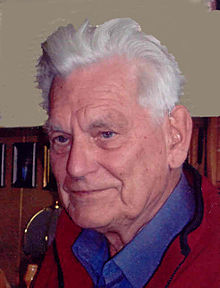
\includegraphics[width=0.9\linewidth]{Images/reenskaug.jpg}
			\end{column}
		\end{columns}
	\end{block}

\end{frame}

\begin{frame}
	\frametitle{Padrões de Projeto para Web}
	\framesubtitle{MVC - Model-View-Controller}

	\begin{figure}
		\centering
		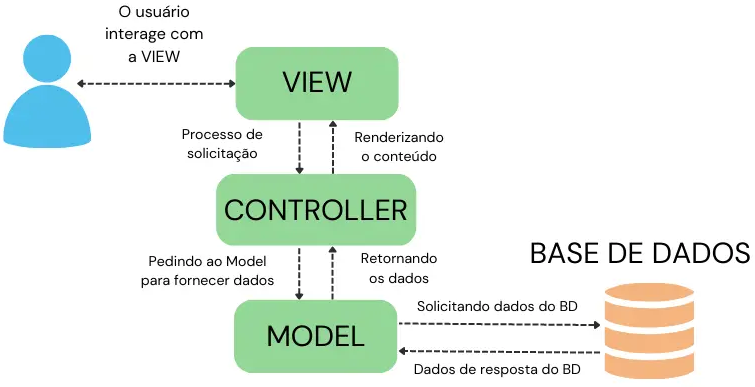
\includegraphics[width=0.9\linewidth]{Images/mvc.png}
		\caption{Estrutura do MVC.}\label{fig:mvc}
	\end{figure}

\end{frame}

\begin{frame}
	\frametitle{Padrões de Projeto para Web}
	\framesubtitle{MVC - Model-View-Controller}

	\begin{block}{Explicando}
		\begin{itemize}
			\item \textbf{Model}: define quais dados o aplicativo deve conter. Se o estado desses dados mudar, o modelo geralmente notificará a visualização (\textit{View}) (para que a exibição possa mudar conforme necessário) e, às vezes, o controlador (se for necessária uma lógica diferente para controlar a visualização atualizada).
			\item \textbf{View}: define como os dados do aplicativo devem ser exibidos (Interface com o Usuário). A visualização é responsável por receber a entrada do usuário e encaminhá-la para o controlador.
			\item \textbf{Controller}: atua como intermediário entre o modelo e a visualização. O controlador é responsável por receber a entrada do usuário da visualização e atualizar o modelo conforme necessário. 
		\end{itemize}
	\end{block}

\end{frame}

% ------------------------------------------------


\subsection{MVP}

\begin{frame}
	\begin{center}
		
		\bigskip\bigskip\bigskip\bigskip % Vertical whitespace
		{\Large Padrões de Projeto}
		
		\bigskip\bigskip % Vertical whitespace
		{\Huge MVP}
		
		\smallskip
		{\small \textit{Model-View-Presenter}}
	\end{center}

\end{frame}

\begin{frame}
	\frametitle{Padrões de Projeto para Web}
	\framesubtitle{MVP - Model-View-Presenter}

	\begin{block}{Definição}
	\begin{columns}[c] % The "c" option specifies centered vertical alignment while the "t" option is used for top vertical alignment
			\begin{column}{0.8\textwidth} % Left column width
				Aborda algumas das desvantagens da abordagem MVC tradicional. Originou-se no início da década de 1990 na Taligent, uma joint venture entre Apple, IBM e Hewlett-Packard. Foi ainda mais popularizado pelo Dolphin Smalltalk em 1998 e, em 2006, a Microsoft adotou o MVP para programação de interface de usuário no framework .NET.
			\end{column}

			\begin{column}{0.2\textwidth} % Right column width
				
\includegraphics[width=0.9\linewidth]{Images/mvp_logo.jpg}
			\end{column}
		\end{columns}
	\end{block}

\end{frame}

\begin{frame}
	\frametitle{Padrões de Projeto para Web}
	\framesubtitle{MVP - Model-View-Presenter}

	No MVP quem manda é o View. Cada View chama seu Presenter ou possui alguns eventos que o Presenter escuta.
	\begin{exampleblock}{Exemplo}
		Quando o usuário clica no botão “Salvar”, o manipulador de eventos na View delega ao método “OnSave” do Presenter. O Presenter fará a lógica necessária e qualquer comunicação necessária com o Modelo e, em seguida, chamará de volta a Visualização por meio de sua interface para que a Visualização possa exibir que o salvamento foi concluído.
	\end{exampleblock}

	
\end{frame}

\begin{frame}
	\frametitle{Padrões de Projeto para Web}
	\framesubtitle{MVP - Model-View-Presenter}

	\begin{figure}
		\centering
		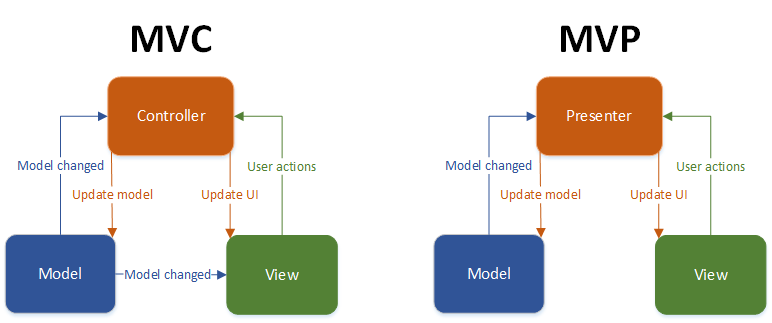
\includegraphics[width=0.9\linewidth]{Images/mvc_mvp.png}
		\caption{Estrutura do MVP.}\label{fig:mvp}
	\end{figure}

\end{frame}

\begin{frame}
	\frametitle{Padrões de Projeto para Web}
	\framesubtitle{MVC vs MVP}

	\begin{block}{MVC vs MVP}
		\begin{itemize}
			\item O \alert{MVC} não coloca o View no comando, os Views atuam como escravos que o Controlador pode gerenciar e direcionar.
			\item No \alert{MVC}, as visualizações são sem estado, ao contrário das visualizações no MVP, onde são com estado e podem mudar com o tempo.
			\item No \alert{MVP}, as Views não têm lógica e devemos mantê-las o mais burras possível. Por outro lado, Views em MVC podem ter algum tipo de lógica.
			\item No \alert{MVP}, o Presenter é desacoplado da View e se comunica com ela através de uma interface. Isso permite que o Presenter seja testado sem a View.
			\item No \alert{MVP}, as visualizações são completamente isoladas do modelo. No entanto, no MVC, as Views podem se comunicar com o Modelo para mantê-lo atualizado.
		\end{itemize}
	\end{block}

\end{frame}

\begin{frame}
	\frametitle{Padrões de Projeto para Web}
	\framesubtitle{MVC vs MVP}

	\centering
	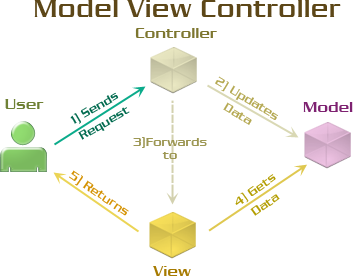
\includegraphics[width=0.5\linewidth]{Images/mvc2.png}
	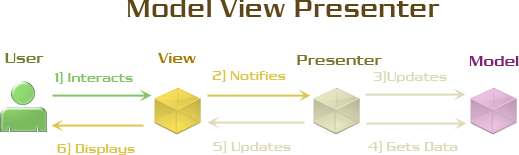
\includegraphics[width=0.8\linewidth]{Images/mvp2.png}

\end{frame}

% ------------------------------------------------

\subsection{MVVM}

\begin{frame}
	\begin{center}
		
		\bigskip\bigskip\bigskip\bigskip % Vertical whitespace
		{\Large Padrões de Projeto}
		
		\bigskip\bigskip % Vertical whitespace
		{\Huge MVVM}
		
		\smallskip
		{\small \textit{Model-View-ViewModel}}
	\end{center}

\end{frame}

% \begin{frame}
% 	\frametitle{Padrões de Projeto para Web}
% 	\framesubtitle{MVVM - Model-View-ViewModel}

% 	\begin{block}{Definição}
% 		É um padrão de Projeto de software que facilita a separação de interesses no desenvolvimento de aplicativos. O MVVM foi criado pelo arquiteto de software do WPF  (Windows Presentation Foundation) e Silverlight da Microsoft, John Grossman em 2005. Desde então, ele vem sendo usado principalmente no desenvolvimento mobile. Ele foi criado para ser usado em aplicativos WPF e usava XAML (uma linguagem declarativa para objetos e suas propriedades) a fim de separar a interface do usuário da lógica de negócios, aproveitando o data binding que é a vinculação de dados.
% 	\end{block}

% \end{frame}

\begin{frame}
	\frametitle{Padrões de Projeto para Web}
	\framesubtitle{MVVM - Model-View-ViewModel}

	O MVVM foi criado pelo arquiteto de software do WPF  (Windows Presentation Foundation) e Silverlight da Microsoft, John Grossman em 2005. Desde então, ele vem sendo usado principalmente no desenvolvimento mobile. Ele foi criado para ser usado em aplicativos WPF e usava XAML (uma linguagem declarativa para objetos e suas propriedades) a fim de separar a interface do usuário da lógica de negócios, aproveitando o data binding que é a vinculação de dados. Na prática, a camada Model não se comunica com a View nem a View se comunica com a Model.

	\begin{block}{Onde é usado?}
		O MVVM é particularmente adequado para aplicativos de \alert{UI complexos}, onde é necessária uma extensa ligação de dados, e para projetos que usam estruturas como WPF, UWP, Angular e Xamarin. Com seu forte foco no desenvolvimento de UI, o MVVM se tornou popular no mundo do \alert{desenvolvimento móvel}.
	\end{block}

	
\end{frame}

\begin{frame}
	\frametitle{Padrões de Projeto para Web}
	\framesubtitle{MVVM - Model-View-ViewModel}

	{\small 
	\begin{itemize}
		\item \textbf{Model}: representa os dados e as regras de negócios. Ele é responsável por recuperar, armazenar e processar dados.
		\item \textbf{View}: é a interface do usuário. Ela é responsável por exibir os dados ao usuário e capturar a entrada do usuário.
		\item \textbf{ViewModel}: é um intermediário entre a View e o Model. Ele é responsável por expor métodos, comandos e outras propriedades que ajudam a manter o estado da View, manipular a entrada do usuário e se comunicar com o Modelo.
		\item \textbf{Data Binding}: é o mecanismo que sincroniza automaticamente a View e o ViewModel. Quando os dados no ViewModel mudam, a View é atualizada automaticamente e vice-versa.
		\item \textbf{Send Notifications}: o ViewModel envia notificações para a View quando os dados mudam. Isso permite que a View saiba quando atualizar a interface do usuário.
	\end{itemize}
	}

	\begin{figure}
		\centering
		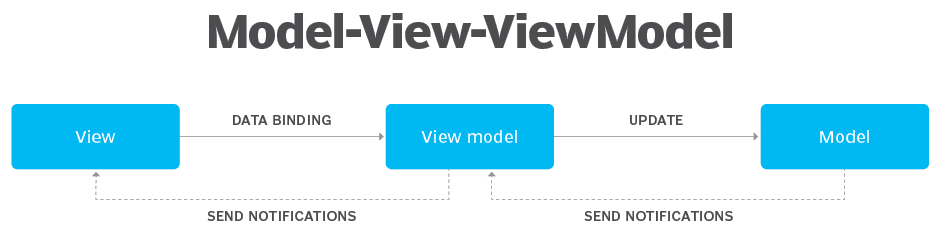
\includegraphics[width=0.9\linewidth]{Images/mvvm.png}
		\caption{Estrutura do MVP.}\label{fig:mvvm}
	\end{figure}

\end{frame}

\section{Material Complementar}

\begin{frame}
	\frametitle{Material Complementar}
	\framesubtitle{Vídeos, Podcasts, Livros, etc}
	
	\begin{itemize}
		\item \iconLink{https://youtu.be/mMDt9g7bMjk}{\textbf{Padrão MVC (Model - View - Controller)}}.\\Canal \textbf{Cod3r Cursos}.\\
		\item \iconLink{https://youtu.be/B2pJWtSyVFA}{\textbf{MVVM (A Arquitetura de Apps Mobile)}}.\\Canal \textbf{Código Fonte TV}.\\
		\item \iconLink{https://www.youtube.com/watch?v=-xTqfilaYow}{\textbf{MVVM in 100 Seconds}}.\\Canal \textbf{Philipp Lackner}.\\
		\item \iconLink{https://www.youtube.com/watch?v=eHhXoCNCI1c}{\textbf{MVC, MVP ou MVVM?}}.\\Canal \textbf{ArjanCodes}.\\
	\end{itemize}
	
\end{frame}

\subsection{Quiz}

\begin{frame}
	\frametitle{Recapitulando}
	\framesubtitle{QUIZ}

	Vamos praticar um pouco o que vimos até agora?
	\vfill

	\bigskip
	\centering

	\iconLink{https://quizizz.com/admin/quiz/659d7e449a88c830fdf1801c?source=quiz_share}{\textbf{QUIZ - Padrões de Projeto MVC, MVP e MVVM}}
	\vfill
		
\end{frame}

% ------------------------------------------------

\section{Tarefa}

\begin{frame}
	\begin{center}
		
		\bigskip\bigskip\bigskip\bigskip % Vertical whitespace
		{\Large Padrões de Projeto}
		
		\bigskip\bigskip % Vertical whitespace
		{\Huge Tarefa}
		
		\smallskip
		{\small \textit{Lista de Exercícios}}

		\bigskip\bigskip
		\begin{block}{Observações}
			\begin{itemize}
				\item As respostas devem ser entregues manuscrítas (escritas à mão).
				\item \textbf{Entrega:} antes do início da próxima aula.
			\end{itemize}
		\end{block}
	\end{center}

\end{frame}

\begin{frame}
	\frametitle{Tarefa}
	\framesubtitle{Lista de Exercícios}
	
	\begin{itemize}
		\item { \small \textbf{Questão 01}: Explique resumidamente o que é um padrão de projeto no contexto web. }
		\item { \small \textbf{Questão 02}: Explique o padrão de projeto MVC (Model-View-Controller). Destaque as responsabilidades de cada componente (Modelo, Visão e Controlador) e como eles interagem para criar uma aplicação estruturada. }
		\item { \small \textbf{Questão 03}: Explique o padrão MVP (Model-View-Presenter) e compare-o com o padrão MVC em termos de responsabilidades e interações entre os componentes. Destaque as vantagens do MVP em cenários específicos. }
		\item { \small \textbf{Questão 04}: Como o padrão MVC aborda a testabilidade em uma aplicação? Compare isso com as estratégias de teste no padrão MVP. Destaque os desafios e benefícios associados à testabilidade em ambos os padrões. }
		\item { \small \textbf{Questão 05}: Explique como a separação de preocupações é alcançada nos padrões MVC, MVP e MVVM. Destaque como essa separação facilita a manutenção do código e a colaboração entre equipes de desenvolvimento. }
		\item { \small \textbf{Questão 06}: Considere um cenário em que a interface do usuário precisa ser atualizada dinamicamente com base em mudanças frequentes nos dados do Modelo. Qual padrão de projeto (MVC, MVP ou MVVM) você escolheria para otimizar a atualização da interface do usuário e por quê? }
	\end{itemize}
	
\end{frame}

% ------------------------------------------------

\begin{frame}
	\begin{center}
		
		\bigskip\bigskip\bigskip\bigskip % Vertical whitespace
		{\Large Padrões de Projeto}
		
		\bigskip\bigskip % Vertical whitespace
		{\Huge Aula 03 - Exemplos e Experimentos Práticos}
		
		\smallskip
		{\small \textit{Lista de Exercícios}}
	\end{center}

\end{frame}


\begin{frame}
	\begin{center}
		
		\bigskip\bigskip\bigskip\bigskip % Vertical whitespace
		{\Large Padrões de Projeto}
		
		\bigskip\bigskip % Vertical whitespace
		{\Huge Exemplos Práticos}
	\end{center}

\end{frame}

\begin{frame}
	\frametitle{Padrões de Projeto para Web}
	\framesubtitle{Exemplo Prático - Sem padrão	de projeto}

	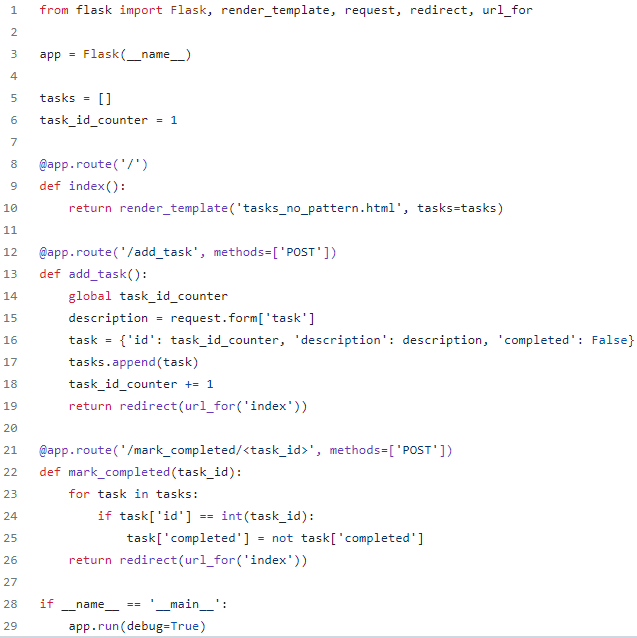
\includegraphics[width=0.6\linewidth]{Images/no_pattern.png}

\end{frame}

\begin{frame}
	\frametitle{Padrões de Projeto para Web}
	\framesubtitle{MVVM - Model-View-ViewModel}

	\begin{block}{Exemplos Práticos}
		\iconLink{https://gist.github.com/fabricioifc/d1bde9f4a13cf63b49870be4bc87a72f}{Exemplo do padrão MVC com Python/Flask}.\\
		\iconLink{https://gist.github.com/fabricioifc/663f8abcba307a013bb56d214752458b}{Exemplo do padrão MVP com Python/Flask}.\\
		\iconLink{https://codepen.io/fabriciobizotto/pen/MWxeONo}{Exemplo do padrão MVVM com VueJS}.
	\end{block}
\end{frame}

% ------------------------------------------------

\section{Experimentos}

\begin{frame}
	\frametitle{Experimentos}
	\framesubtitle{Lista de Exercícios}
	
	\begin{itemize}
		\item \textbf{Experimento 01}
		\begin{itemize}
			\item Modifique o exemplo do padrão MVC para adicionar a funcionalidade de \textbf{excluir} uma tarefa, ou
			\item Modifique o exemplo do padrão MVP para adicionar a funcionalidade de \textbf{excluir} uma tarefa, ou
			\item Modifique o exemplo do padrão MVVM para adicionar a funcionalidade de \textbf{excluir} uma tarefa.
		\end{itemize}
			\item \textbf{Experimento 02}
			\begin{itemize}
				\item Crie outro exemplo simples de aplicação web utilizando o padrão MVC, MVP ou MVVM para demonstrar o funcionamento do padrão.
			\end{itemize}
	\end{itemize}

	\begin{block}{Observações}
		\begin{itemize}
			\item Os experimentos devem ser publicados no \textbf{GitHub}. No arquivo \textbf{README.md}, explique resumidamente o que foi feito e como foi feito.
			\item \textbf{Entrega:} à combinada com o professor.
			\item \textbf{Avaliação:} Faz parte da 1° avaliação.
		\end{itemize}
		\alert{Faremos uma aula para compartilhar os experimentos e discutir os resultados.}
	\end{block}
	
\end{frame}

%------------------------------------------------

% \subsection{Columns}

% \begin{frame}
% 	\frametitle{Multiple Columns}
% 	\framesubtitle{Subtitle} % Optional subtitle
	
% 	\begin{columns}[c] % The "c" option specifies centered vertical alignment while the "t" option is used for top vertical alignment
% 		\begin{column}{0.45\textwidth} % Left column width
% 			\textbf{Heading}
% 			\begin{enumerate}
% 				\item Statement
% 				\item Explanation
% 				\item Example
% 			\end{enumerate}
% 		\end{column}
% 		\begin{column}{0.5\textwidth} % Right column width
% 			Lorem ipsum dolor sit amet, consectetur adipiscing elit. Integer lectus nisl, ultricies in feugiat rutrum, porttitor sit amet augue. Aliquam ut tortor mauris. Sed volutpat ante purus, quis accumsan dolor.
% 		\end{column}
% 	\end{columns}
% \end{frame}

% %------------------------------------------------

% \section{Table and Figure Examples}

% \subsection{Table}

% \begin{frame}
% 	\frametitle{Table}
% 	\framesubtitle{Subtitle} % Optional subtitle
	
% 	\begin{table}
% 		\begin{tabular}{l l l}
% 			\toprule
% 			\textbf{Treatments} & \textbf{Response 1} & \textbf{Response 2}\\
% 			\midrule
% 			Treatment 1 & 0.0003262 & 0.562 \\
% 			Treatment 2 & 0.0015681 & 0.910 \\
% 			Treatment 3 & 0.0009271 & 0.296 \\
% 			\bottomrule
% 		\end{tabular}
% 		\caption{Table caption}
% 	\end{table}
% \end{frame}

% %------------------------------------------------

% \subsection{Figure}

% \begin{frame}
% 	\frametitle{Figure}
	
% 	\begin{figure}
% 		
\includegraphics[width=0.8\linewidth]{logo.png}
% 		\caption{IFC Videira.}
% 	\end{figure}
% \end{frame}

% %------------------------------------------------

% \section{Mathematics}

% \begin{frame}
% 	\frametitle{Definitions \& Examples}
	
% 	\begin{definition}
% 		A \alert{prime number} is a number that has exactly two divisors.
% 	\end{definition}
	
% 	\smallskip % Vertical whitespace
	
% 	\begin{example}
% 		\begin{itemize}
% 			\item 2 is prime (two divisors: 1 and 2).
% 			\item 3 is prime (two divisors: 1 and 3).
% 			\item 4 is not prime (\alert{three} divisors: 1, 2, and 4).
% 		\end{itemize}
% 	\end{example}
	
% 	\smallskip % Vertical whitespace
	
% 	You can also use the \texttt{theorem}, \texttt{lemma}, \texttt{proof} and \texttt{corollary} environments.
% \end{frame}

% %------------------------------------------------

% \begin{frame}
% 	\frametitle{Theorem, Corollary \& Proof}
	
% 	\begin{theorem}[Mass--energy equivalence]
% 		$E = mc^2$
% 	\end{theorem}
	
% 	\begin{corollary}
% 		$x + y = y + x$
% 	\end{corollary}
	
% 	\begin{proof}
% 		$\omega + \phi = \epsilon$
% 	\end{proof}
% \end{frame}

% %------------------------------------------------

% \begin{frame}
% 	\frametitle{Equation}

% 	\begin{equation}
% 		\cos^3 \theta =\frac{1}{4}\cos\theta+\frac{3}{4}\cos 3\theta
% 	\end{equation}
% \end{frame}

% %------------------------------------------------

% \begin{frame}[fragile] % Need to use the fragile option when verbatim is used in the slide
% 	\frametitle{Verbatim}
	
% 	\begin{example}[Theorem Slide Code]
% 		\begin{verbatim}
% 			\begin{frame}
% 				\frametitle{Theorem}
% 				\begin{theorem}[Mass--energy equivalence]
% 					$E = mc^2$
% 				\end{theorem}
% 		\end{frame}\end{verbatim} % Must be on the same line
% 	\end{example}
% \end{frame}

% %------------------------------------------------


% \section{Referências}

% \begin{frame}
% 	\frametitle{Referências}
% 	\printbibliography
% \end{frame}

%----------------------------------------------------------------------------------------
%	CLOSING SLIDE
%----------------------------------------------------------------------------------------

% \begin{frame}[plain] % The optional argument 'plain' hides the headline and footline
% 	\begin{center}
% 		\bigskip\bigskip % Vertical whitespace
		
% 		{\Huge Perguntas? Comentários?}
		
% 		\bigskip\bigskip % Vertical whitespace
		
% 		{\LARGE Aula 03 - Padrões de Arquitetura}
% 	\end{center}
% \end{frame}

%----------------------------------------------------------------------------------------

\end{document} 